%! TEX root = ../../main.tex

\subsection{Automation of a Microservice's Deployment}%
\label{sub:Automatic_a_Microservices_Deployment}
So far this thesis already introduced the concept of microservices and how they
can be deployed using a container orchestration solution; in the case of this
thesis Kubernetes. Yet, the deployment options offered in
chapter~\ref{sub:Kubernetes} all have to executed by hand. Additionally
chapter~\ref{sub:Kubernetes} presupposes that the container's image is already
available on a central image repository. The basic Docker development workflow
as shown in figure~\ref{fig:docker_workflow} also assumes that developers
manually build the service's image on their local machine and push them to the
central repository. While this is still a valid possibility, the process
consumes a lot of extra time spent by the developer and is error prone.
Furthermore, in such a manual process no central quality control can force
policies upon the source code of each service. These problems can be solved by
introducing an additional automation component: A \acf{CI} and \ac{CD} server.
This section will outline the basic principles of such a server and apply them
to the exemplary \ac{SaaS} solution \textit{Microsoft DevOps}.

\subsubsection{Continuous Integration}%
\label{ssub:Continuous_Integration}
The basis for continuously releasing a software, in this case a microservice,
is a \ac{CI} concept. This concept spans a wide range of topics including the
\begin{itemize}
  \item compilation of source code,
  \item integration of databases,
  \item execution of tests,
  \item application of rules upon the source code using inspection and
  \item preparation of documentation and feedback of each build \autocite[pp.
    12-20]{MatyasContinuousIntegration2007}.
\end{itemize}

\autocite{MatyasContinuousIntegration2007} also includes the continuous
deployment of software though this will be covered separately in the next
passage, chapter~\ref{ssub:Continuous_Deployment}. Each iteration of the steps
listed above is called a \textit{build}. A build assembles the source code and
makes sure that the software works as intended \autocite[p.
4]{MatyasContinuousIntegration2007}. The \textit{integration} of software
usually consists of the steps portrayed in
figure~\ref{fig:ci_pipeline_classic}. The whole process is also often referred
to as being a \textit{pipeline}.

\begin{figure}[H]
\begin{center}
  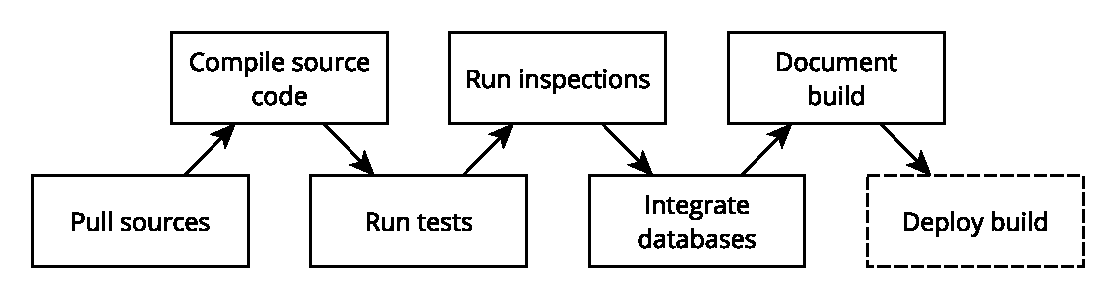
\includegraphics[scale=0.7]{images/figures/ci_classic.pdf}
\end{center}
\caption[The most common, abstracted \ac{CI} pipeline for a classic
software.]{The most common, abstracted \ac{CI} pipeline for a classic
software (adapted from \autocite[Fig. 1-4]{MatyasContinuousIntegration2007}).}%
\label{fig:ci_pipeline_classic}
\end{figure}
\todo{The order of steps may has to be adjusted (position of compilation).}

In order for this pipeline to be implemented, a number of prerequisites exist.
\autocite{MatyasContinuousIntegration2007} and
\autocite{JezHumbleContinuousDelivery2010} outline that

\begin{itemize}
  \item all code has to be tracked in a central \ac{VCS},
  \item changes have to be checked in regularly,
  \item an extensive, automated test suite has to be in place and
  \item the software has to be buildable and testable in any environment.
\end{itemize}

First, the project's source code has to be tracked in a \ac{VCS}. The \ac{VCS}
holds the source code in a central place that can be accessed by all developers
\autocite[Ch.  1]{MatyasContinuousIntegration2007}. In addition, the \ac{VCS}
allows multiple developers to work on different tasks for the same project
concurrently. The \ac{VCS} acts as the data foundation for the integration
process.

Furthermore, the code produced by the developers has to be checked in the
\ac{VCS} regularly. Only then may the \ac{CI} process detect problems early and
inform the responsible developer of the breaking change. Code should be checked
in more than a couple of times a day \autocite[p.
59]{JezHumbleContinuousDelivery2010}. \todo{Maybe add statement that states
that CI is not compatible with branching; Maybe refute?}

A requirement for successful continuous integration is an extensive test suite.
When building software, a successful build does not necessarily imply that the
software works as indented. E.g.\ a calculator service might compile but as
long as the addition function returns \texttt{1 + 1 = 3}, the code should not be
classified as performing correctly. The test suites must also be able to be
executed automatically \autocite[p. 60]{JezHumbleContinuousDelivery2010}.

\autocite[p. 62]{JezHumbleContinuousDelivery2010} further states that the
developers should be able to build and test the software in any environment
under their control; including their local machine. This is particularly well
feasible when working with microservices that will eventually be deployed to a
Kubernetes cluster. Kubernetes is not only able to run in a datacenter but also
on a developer's machine.

As long as all these requirements are fulfilled, a \ac{CI} process can be
successfully used. Though when applying \ac{CI} to microservice architectures,
an additional remark needs to be made. The traditional \ac{CI} process does
not specify how the software should be build \autocite[p.
18]{MatyasContinuousIntegration2007}. In a monolithic project, a usual outcome
of the \ac{CI} process is a bundle of the built software that also includes all
database schemas and installation scripts. This piece of data is also referred
to as an \textit{artefact} \autocite[p. 18]{MatyasContinuousIntegration2007}.
As outlined in chapter~\ref{ssub:Dockerizing_a_Microservice}, microservices are
shipped as Docker images. Thus a successful build process always has to produce
a Docker image and push it to a central image repository. The \ac{CI} artefact
in a microservice project hence would be a runnable Docker image. That Docker
image bundles the full runtime environment and thus does not need to include
the installation instructions and scripts.

\begin{figure}[H]
\begin{center}
  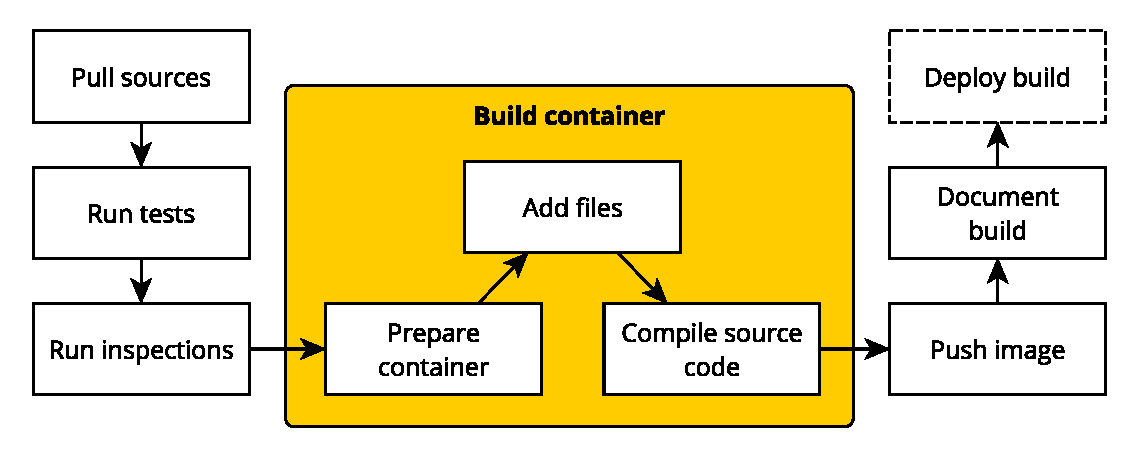
\includegraphics[scale=0.7]{images/figures/ci_container.pdf}
\end{center}
\caption{The \ac{CI} pipeline for a containerized project.}%
\label{fig:container_ci_pipeline}
\end{figure}

As shown in figure~\ref{fig:container_ci_pipeline}, the software is no longer
compiled on the machine running the \ac{CI} pipeline. The compilation now takes
place inside the Docker build process. The reasons for this are further
outlined in the upcoming section~\ref{ssub:Continuous_Deployment}. Another
distinction between the classic \ac{CI} pipeline from
figure~\ref{fig:ci_pipeline_classic} to the dockerized model from
figure~\ref{fig:container_ci_pipeline} is that the build artefact no longer
only remains on the build machine. After an image was successfully constructed,
it is pushed to a central image repository for further use.

\subsubsection{Continuous Deployment}%
\label{ssub:Continuous_Deployment}
Now that the \ac{CI} process has produced a runnable artefact, the next step is
to deploy this artefact to an environment. The environment to which the
artefact is deployed can be freely chosen. However the most typical
environments a software lives in are outlined in the upcoming
chapter~\ref{sub:Deployment_Environments}. In general \ac{CD} is a set of
methods and steps that deploys software scheduled to an end user. A software
that is not successfully deployed does not exist for the end user. \ac{CD}
helps developers to overcome this problem by giving them a framework for
automating this process \autocite[pp. 190]{MatyasContinuousIntegration2007}.

The need for automating the deployment process becomes clear when taking a look
at Amazon. Amazon deploys its software approx.\ every 11.6 seconds. This
statistic only includes deployments to production and does not cover Amazon's
other deployment environments like development
\autocite{JenkinsVelocityCulture2011}. When encompassing this sheer amount of
releases and such short release cycles it becomes clear that deployments have
to be automated.

To successfully implement \ac{CD}, a number of requirements have to be
fulfilled:
\begin{itemize}
  \item Labels have to be applied to the files inside the \ac{VCS}
    \autocite[pp. 191-194]{MatyasContinuousIntegration2007}.
  \item Labels have to be applied to each build \autocite[pp.
    195f.]{MatyasContinuousIntegration2007}.
  \item The environment to which the software will be deployed has to be
    \textit{clean} \autocite[pp. 194f.]{MatyasContinuousIntegration2007}.
  \item All tests must pass in order for a software to be declared working
    \autocite[p. 196]{MatyasContinuousIntegration2007}.
  \item A feedback report has to be created at the end of each build
    \autocite[pp. 196-198]{MatyasContinuousIntegration2007}.
  \item Releases must be able to be rolled back \autocite[p.
    199]{MatyasContinuousIntegration2007}.
\end{itemize}

Labels should be applied to both files stored inside the \ac{VCS} as well as
the outcome of each build. Files with the same label can be considered to be a
group. Further, in the worst case, labels allow software to be rolled back
easily without having to track the files of a release individually. A new
release from the same files can be created with ease when all files are tracked
with a label \autocite[pp. 191-194]{MatyasContinuousIntegration2007}.

Build labels on the other hand do not track uncompiled files. They are applied
to the artefacts of a build and are unique. Hence, a build artefact produced
from a snapshot of files e.g.\ labelled \texttt{release\textunderscore 2.0.1}
could be labelled \texttt{release\textunderscore 2.0.1-\textbf{1}}. Each time
the artefact is rebuilt, the last number at the end of the label (\texttt{1})
is incremented. When using a labelled build the features, defects and
requirements can be traced to a specific release version. Without
labels it would not be possible to e.g.\ pin issues to an explicit release
\autocite[pp. 195f.]{MatyasContinuousIntegration2007}.

In addition, a \textit{clean} environment has to be provided for each
deployment. That means that no leftover files from other deployments are still
present on a machine when the next deployment is applied. Any leftover files
may distort the execution of the software and thus may mask or provoke unwanted
behaviour. \autocite{ArtacDevOpsIntroducingInfrastructure2017} offers a
layer-based approach to avert this problem. In this approach a \textit{machine}
is composed of multiple \textit{layers}. Each layer is stacked on top of the
previous one and together they build the environment in which the application
is executed. The layers range from the \ac{OS}, its configuration files, any
middleware components (like an application server) or additional pieces of
software (like a database server) up to the actual software. Each time a new
deployment is applied, the complete stack is purged and rebuilt from the ground
up \autocite[p. 194]{MatyasContinuousIntegration2007}.

In a monolithic architecture this approach might suffice. However, it has to be
adapted to also support a containerized microservice architecture. First of
all, each time a container for a microservice is created, only a few layers on
top of the stack are rebuilt. When e.g.\ deploying an application that depends
on a \textit{NGINX} web server, the web server and any underlying layers can be
reused as part of a Docker base image. So only the layers on top of the web
server have to be reapplied. This process also ensures that the environment to
which the software is deployed is clean while being more efficient than
rebuilding each layer. In addition, the use of a container orchestration
solution like Kubernetes has the advantage of defining the underlying
infrastructure as code. \ac{IaC} allows the infrastructure to be defined inside
a \enquote{single commonly available source of truth}, most frequently stored
inside a \ac{VCS}, without the need for additional administrators
\autocite{ArtacDevOpsIntroducingInfrastructure2017}. In Kubernetes,
infrastructure changes can be performed by applying these configuration files.
When implemented correctly, the developer performing these changes does not have
to worry about past infrastructure configurations remaining in the system.
Kubernetes keeps track of old resources and manages them accordingly
\autocite{AuthorsDeployments2019}. The \ac{IaC} paradigm further supports the
aim of always producing a clean deployment environment.

It is a common approach to run tests locally before pushing code changes to the
\ac{VCS}. The local environment however most often differs, even if only in
minor details, from the actual environment the application will be deployed in.
Hence, it can not be guaranteed that a passing test on the local machine also
produces the same result in the deployment environment. This is the reason why
\textit{all} tests also have to be completed in the deployment environment. The
tests do not only have to be executed, all tests need to pass. Only then it can
be guaranteed that the software is working as expected \autocite[p.
196]{MatyasContinuousIntegration2007}. As already shown in
figure~\ref{fig:container_ci_pipeline} the source code is compiled inside a
container. Docker has the option of multi-stage builds. In a multi-staged
build, the container creation is split into multiple stages. Each stage has
random access to the file system of any other stage. Using this approach it is
e.g.\ possible to create a stage in which the software is built that has the
needed compiler set up. An additional stage could then copy the compiled binary
into an environment which has no compiler installed. As a result the final
container image becomes smaller while only containing data for the execution of
the software \autocite{IncUsemultistage2019}. The same thought can be applied
to tests. Before compiling, a separate stage holds all test utilities needed to
test the software. The tests are executed a second time and the build pipeline
only proceeds if all tests pass a second time inside that specialised early
build stage.

\begin{figure}[H]
\begin{center}
  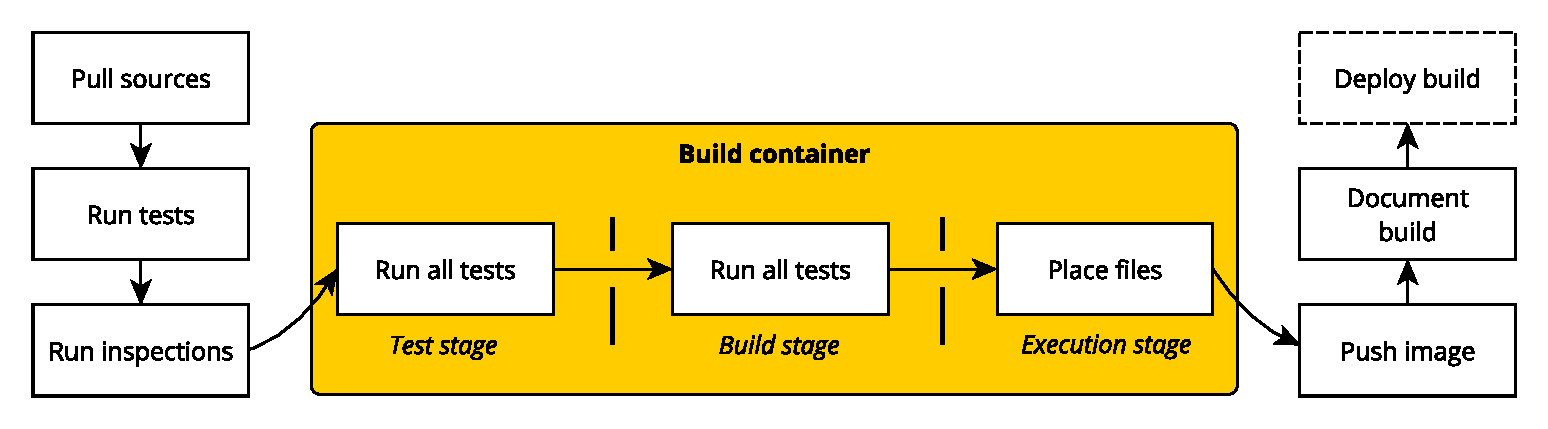
\includegraphics[scale=0.6]{images/figures/ci_container_extended.pdf}
\end{center}
\caption{Re-execution of the tests during the Docker build process in a
containerized project.}%
\label{fig:container_ci_pipeline_extended}
\end{figure}

Regardless of the outcome of the build, a feedback report should be generated.
That report includes information about the changed files, new features and
fixes. Any interested team member can then verify whether the build contains
the desired aspects \autocite[pp. 196-198]{MatyasContinuousIntegration2007}.

Lastly the \textit{Cloudflare} outage in July 2019 showed the importance of
having a working process in place to roll back any release. Even though
Cloudflare had a rollback plan in place, they could not successfully execute
it. This resulted in a unavailability of Cloudflare's global network for 27
minutes stranding nearly all of their customers
\autocite{Graham-CummingDetailsCloudflareoutage2019}. The existence of a
working and fast rollback process allows defects introduced by a release to be
temporarily resolved by simply rolling back to the previous version
\autocite[p. 199]{MatyasContinuousIntegration2007}.

Given that these requirements are fulfilled, it is ensured that the automated
build produces a working software that can be released at any time \autocite[p.
200]{MatyasContinuousIntegration2007}.

\subsubsection{Azure DevOps}%
\label{ssub:Azure_DevOps}
Now that the foundation for the understanding of how microservices can be
continuously integrated and deployed is laid, the explored principles can be
put into practise. Previously, chapter~\ref{ssub:Continuous_Integration}
and~\ref{ssub:Continuous_Deployment} already mentioned a \textit{machine} on
which a build is executed. A machine however is not sufficient for implementing
a \ac{CI}/\ac{CD} pipeline. An additional piece of software is needed that
knows how to run the pipeline and its various steps. One of these solutions is
called \textit{Microsoft Azure DevOps}. This section will outline how Azure
DevOps implements the previously explored features of \ac{CI}/\ac{CD}.

To understand the upcoming solution by Microsoft, a short definition of the
term \textit{DevOps} might be beneficial. For a long time, the tasks of
developing and operating an application was clearly segregated. A development
team implemented an application and an operations team operated the application
and the underlying infrastructure. DevOps aims to reduce the distance between
these two practises. It defines a number of socio-technical and organizational
methods which bit by bit reduce that distance. This means that development
teams are encouraged to engage with the operational aspects of their
application until ultimately the development and operation teams blend
together. This is supported by DevOps tools that are shared between the
development and operation teams (e.g.\ a common documentation) in order to
avoid knowledge gaps \autocite{ArtacDevOpsIntroducingInfrastructure2017}.

With Azure DevOps, Microsoft introduced a solution that equips teams following
the DevOps methodology with various tools. The tools included with Azure DevOps
are listed in table~\ref{tab:azure_devops}.

\LTXtable{\textwidth}{tables/azure_devops.tex}

Though all of the tools listed in table~\ref{tab:azure_devops} aid teams in
continuously releasing a microservice architecture, the upcoming section will
only examine \textit{Azure Pipelines}, Microsoft's \ac{CI}/\ac{CD} solution.

Azure Pipelines consists of the two main modules \textit{Builds} and
\textit{Releases}. These two make up Azure DevOps' \ac{CI} and \ac{CD}
capabilities. In addition to these two, Azure Pipelines includes a
\textit{Library} feature that can store groups of variables secure files like
signing keys. \textit{Task groups} allow users to define common deployment
steps in a central place. This can be helpful if the same set of steps is
required in multiple build pipelines (e.g.\ a Node.js application always needs
to install its dependencies first and then build the code). Lastly,
\textit{Deployment groups} can be used to configure groups of machines, e.g.\ a
development cluster, to which a release can be deployed. As the Library, Task
Groups and Deployment Groups features only contribute advanced capabilities for
the Build and Releases features, they will not be explored further at this
point.

Pipelines are made up of one or more \textit{Stages}. Each stage can contain
two types of tasks: \textit{Jobs} and \textit{Deployments}. Even though it is
possible to realise deployment tasks using a Job, Microsoft discourages this
behaviour and recommends the use of Deployments instead. Deployments e.g.
preserve a history of Deployments that would not be collected when using Jobs.
Further, it possible to define one or more Jobs and Deployments per Stage. Both
Jobs and Deployments can contain multiple steps. DevOps treats different types
of Steps differently. The types \texttt{script}, \texttt{bash}, \texttt{pwsh}
and \texttt{powershell} each run commands a respective shell whereas
\texttt{checkout}, \texttt{task} and \texttt{templateReference} perform
additional pipeline and repository related actions. Jobs and Deployments may
require that preconditions be fulfilled before running. This allows developers
to e.g.\ integrate manual reviews into a pipeline \autocite{MicrosoftJobs2019}.

\begin{figure}[H]
\begin{center}
  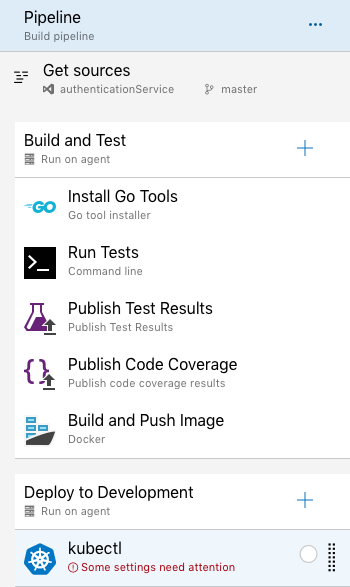
\includegraphics[scale=0.6]{images/figures/azure_devops_build_pipeline.png}
\end{center}
\caption{A build pipeline in Microsoft Azure DevOps.}%
\label{fig:build_pipeline_azure}
\end{figure}

Traditionally, build pipelines could only be created and modified in a visual
editor. Figure~\ref{fig:build_pipeline_azure} shows an exemplary Azure DevOps
pipeline that consists of the two Jobs \texttt{Build and Test} and
\texttt{Deploy to Development}. The first Job has five Steps and the second Job
one Step.

\begin{figure}[H]
\begin{center}
  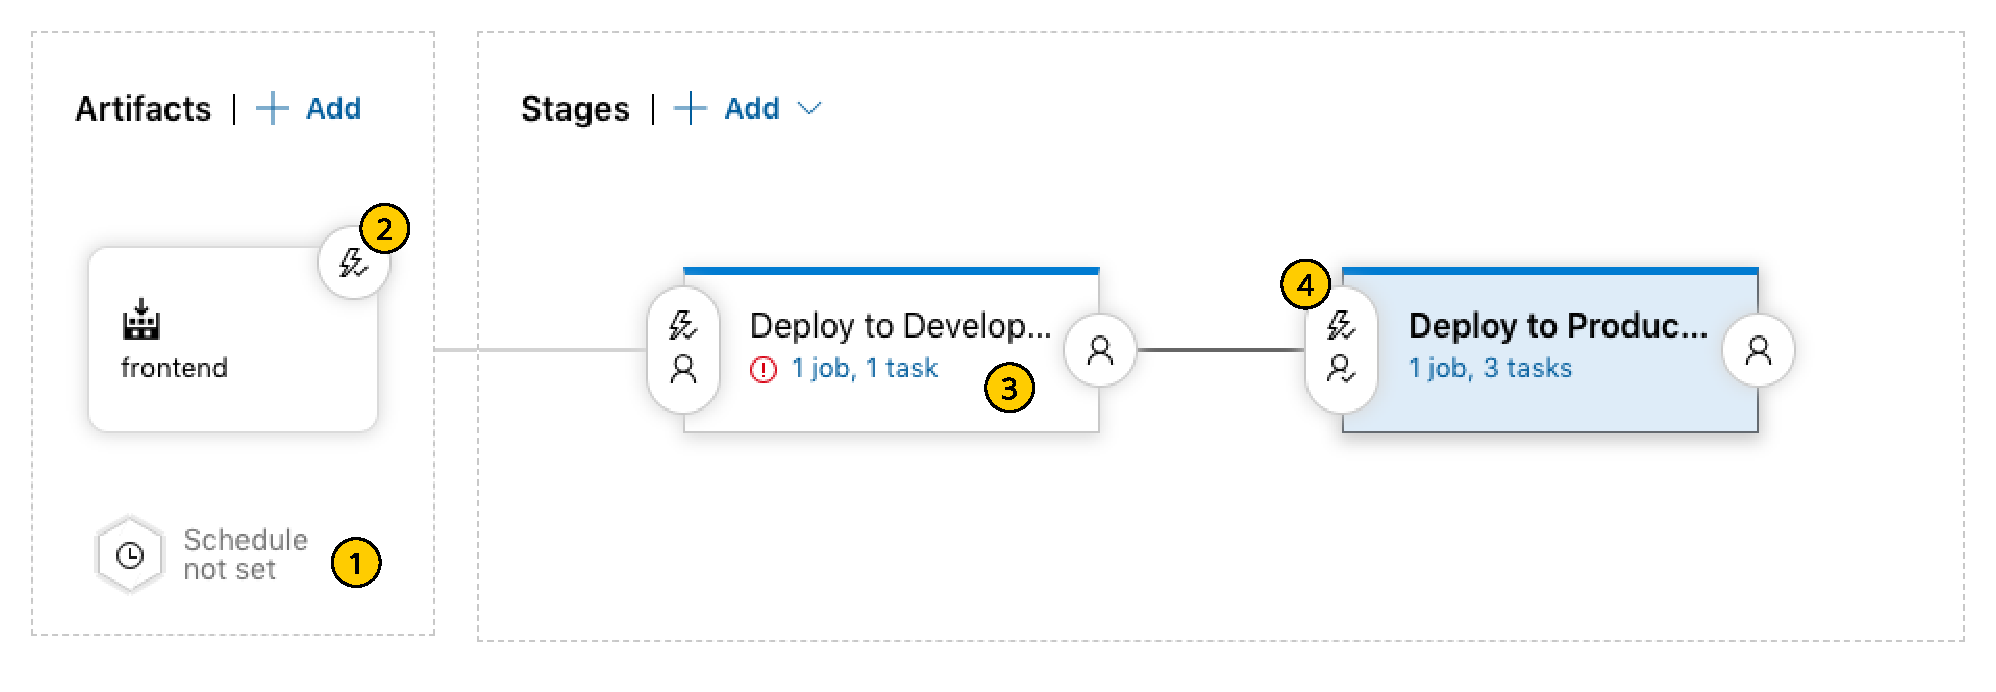
\includegraphics[scale=0.5]{images/figures/azure_devops_release_pipeline_base.pdf}
\end{center}
\caption{A release pipeline in Microsoft Azure DevOps.}%
\label{fig:release_pipeline_azure}
\end{figure}

Like build pipelines, release pipelines could traditionally only be set up in a
graphical user interface. Figure~\ref{fig:release_pipeline_azure} shows a
release pipeline with two stages that are not executed on a schedule
(\circled{1}) but every time a new artefact called \texttt{frontend} is created
(\circled{2}). \circled{3} shows a deployment stage in which the application is
deployed to a development environment. To do this, only one task is needed.
After the application was successfully deployed to development, the deployment
to the production environment is triggered. This however is put on hold until
an approval is given as indicated by \circled{4}.

When using the visual release pipeline editor, the build process if fully
decoupled from the release process. It only acts as a trigger for the release
pipeline and is defined in a fully separate interface
(figure~\ref{fig:build_pipeline_azure}).

In newer versions of Azure DevOps, the configuration via YAML files is
preferred. Though until Azure DevOps' update in July 2019 it was not possible
to define multi-stage pipelines, meaning pipelines that build and release a
software, in one common YAML file. With the introduction of file-defined,
multi-stage pipelines, the graphical configuration interface for pipelines can
be entirely discarded. The pipeline configuration is stored next to the
application's actual code inside a \ac{VCS}. In a microservice environment of
$n$ microservices, $n$ pipeline configuration files would be stored in each
microservice's code repository. This allows for a cleaner versioning of build
and deployment configurations right next to the project's code.

\begin{listing}
\begin{minted}{YAML}
stages:
- stage: BuildAndTest
  jobs:
    - job: ...
- stage: DeployToDevelopment
  dependsOn: BuildAndTest
  condition: succeeded('BuildAndTest')
- stage: DeployToProduction
  dependsOn: Development
  condition: succeeded('DeployToDevelopment')
\end{minted}
\caption{A build and release pipeline (multi-staged) in Microsoft Azure DevOps.}
\label{lst:multi_stage_azure}
\end{listing}

In listing~\ref{lst:multi_stage_azure}, an exemplary multi-stage pipeline
configuration file is shown. Like in the graphical interface, a stage can
appoint another stage as its predecessor. When doing so, the appointing stage
is only executed after the predecessor's run is completed. In addition, a stage
can require that certain conditions are fulfilled. If a condition fails, the
stage defining it is not executed.

Even if multi-stage pipeline configuration files are an improvement over the
graphical configuration, the feature is still in a preview phase. Hence, not
all features available in the graphical editor are already ported to be used
inside the YAML-based configurations.
